% =====================================================================
\chapter{Modelo cinemático, jacobiano y modelo 3D}\label{cap:cinematica}

\section{Levantamiento de medidas}
El modelo parte de un levantamiento de la máquina: 20 fotos acotadas (\codigo{modelo-3d/levantamiento/fotos/}), bocetos de las piezas, una planilla de medición imprimible y el manual del fabricante. Cada cota quedó clasificada: \emph{leída} (medida en la pieza o el boceto), \emph{estimada} (de fotos o del manual, ajustada para que el modelo reproduzca las fotos con menos de 5~mm de diferencia) o \emph{SUPUESTO}.

\begin{figure}[H]
\centering
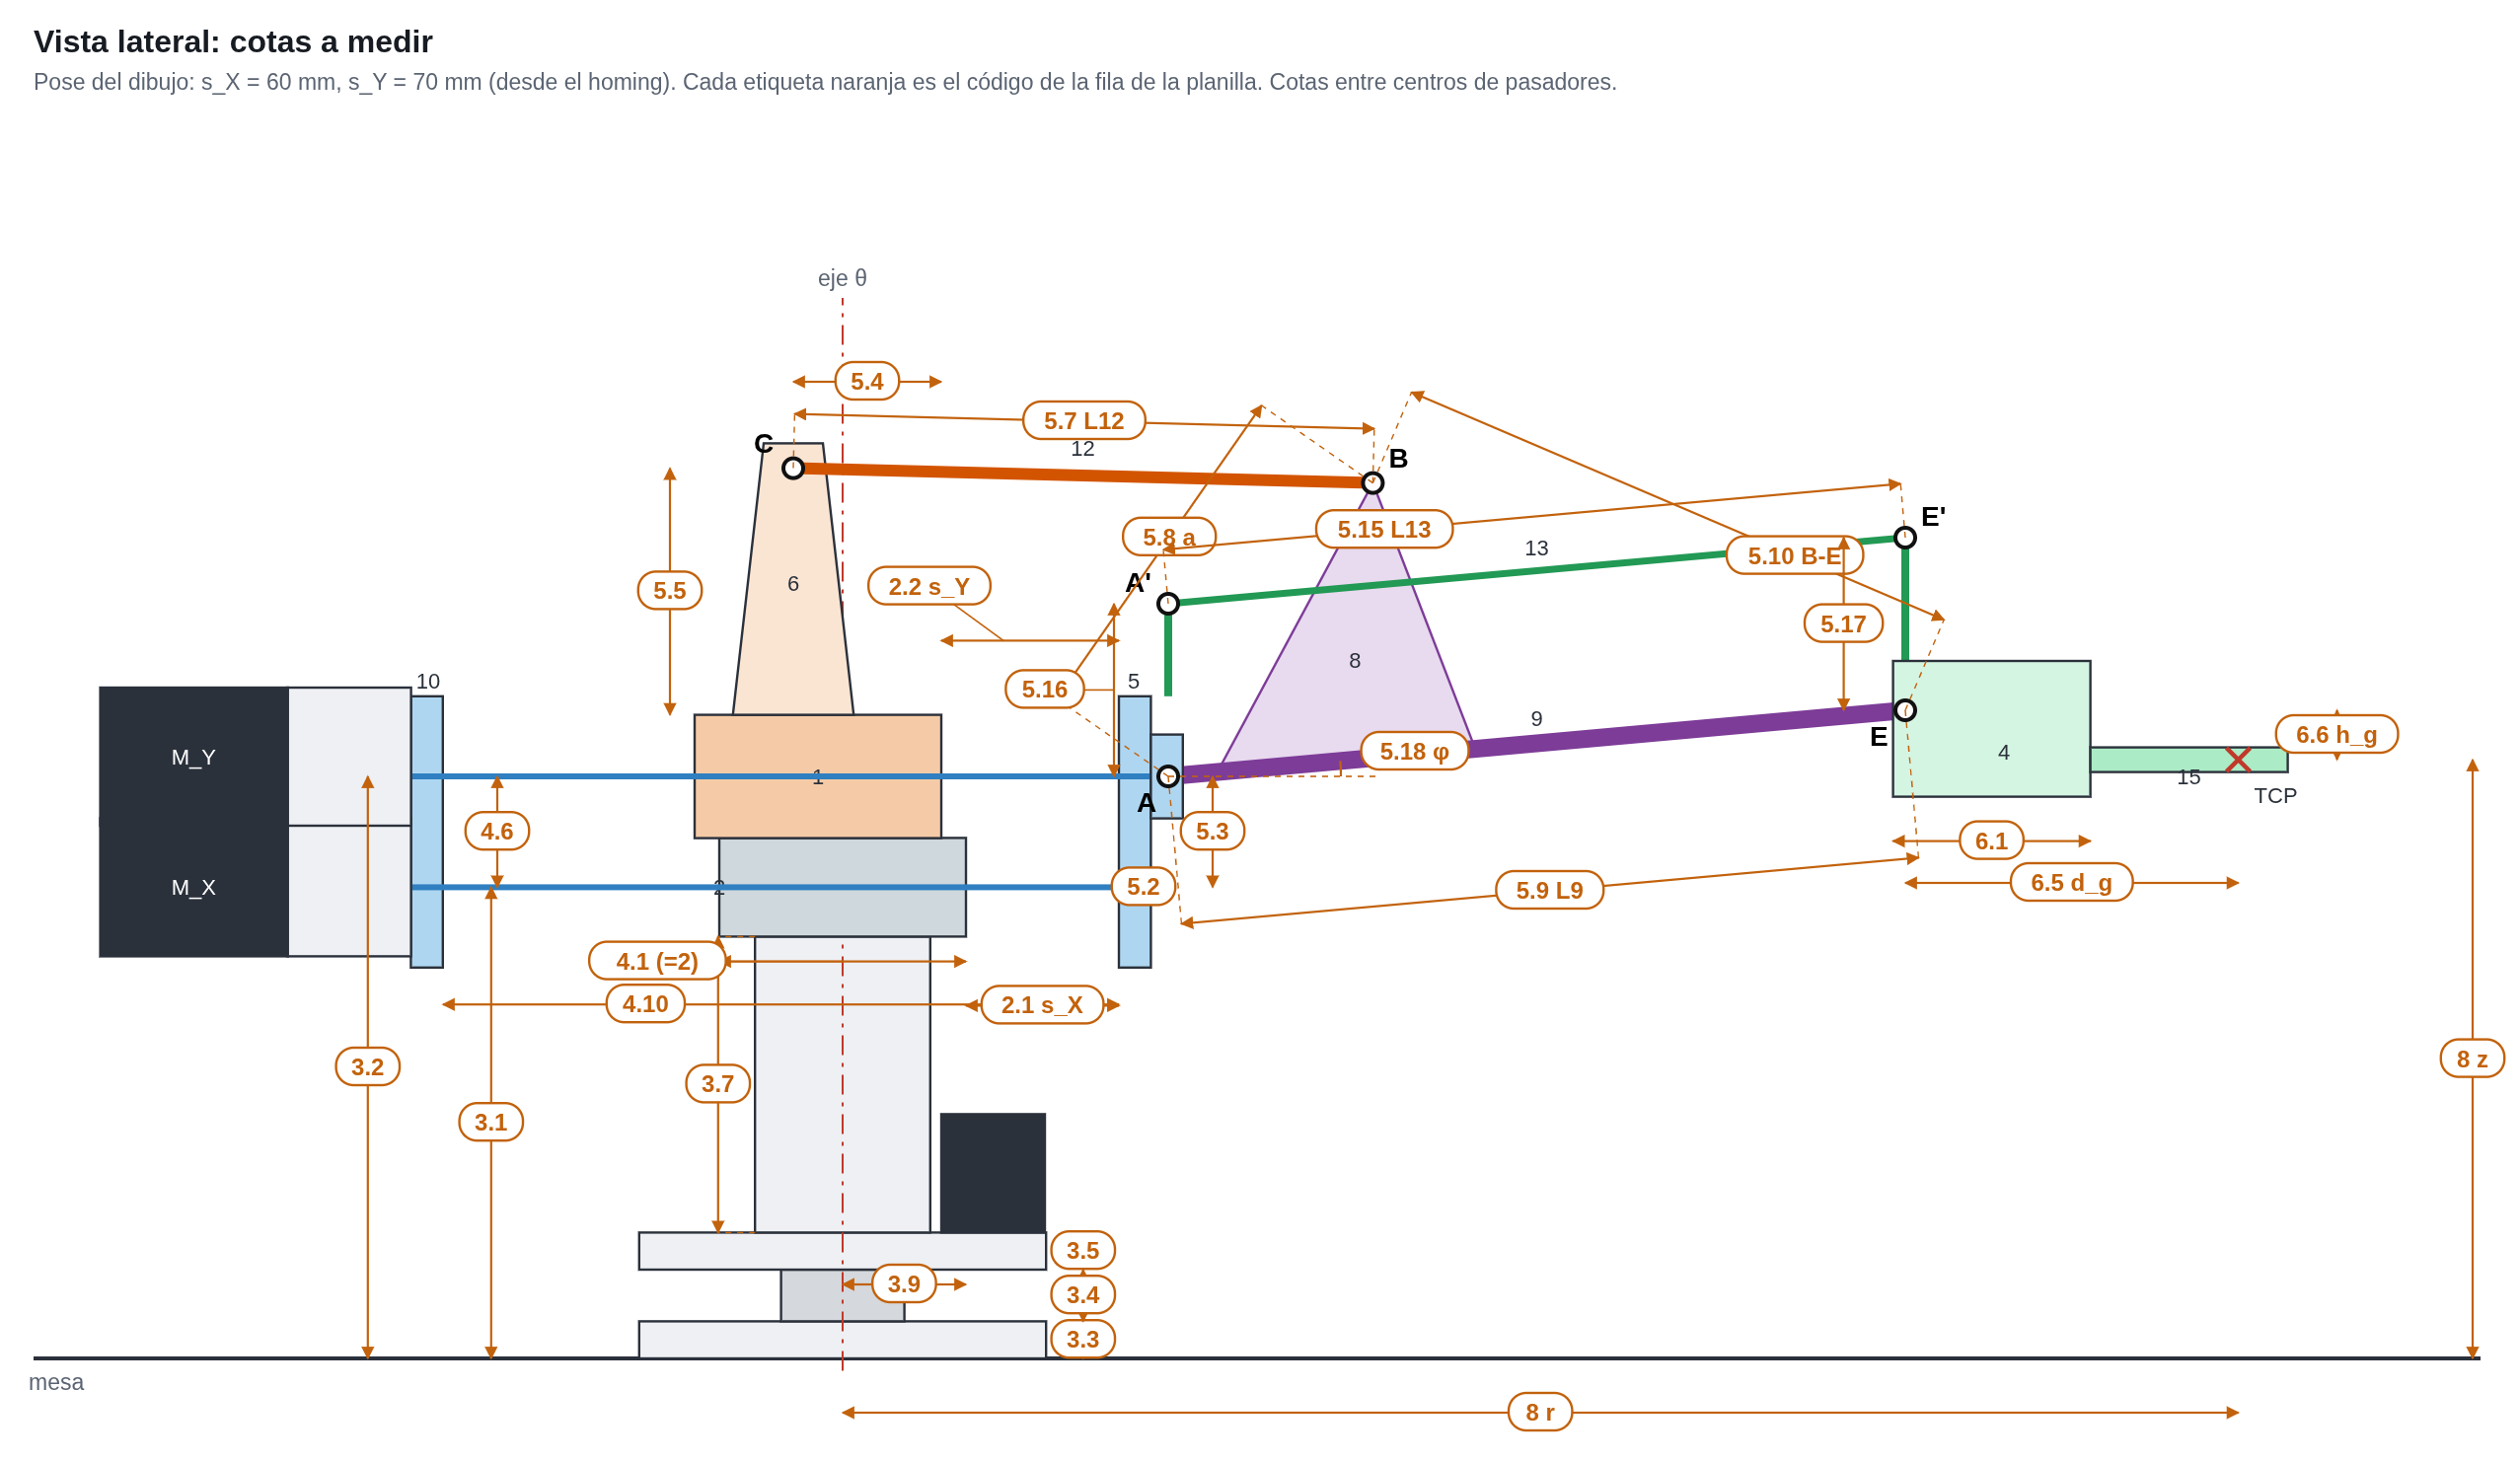
\includegraphics[width=\linewidth]{esquema_medidas_lateral.png}
\caption{Esquema de medidas en vista lateral (\texttt{levantamiento/esquema\_medidas\_lateral.png}).}
\end{figure}

\begin{center}\small
\begin{longtable}{>{\ttfamily}p{2.6cm} r >{\raggedright}p{2cm} >{\raggedright\arraybackslash}p{8cm}}
\toprule
\textbf{\rmfamily Parámetro} & \textbf{Valor} & \textbf{Origen} & \textbf{Significado}\\
\midrule
\endhead
largoGuias & 300 mm & leída & guías del bastidor\\
espesorPlaca & 13 mm & leída & placas extremas del bastidor\\
largoBloque & 100 mm & leída & bloques 1 y 2\\
holgura & 2 mm & SUPUESTO & distancia bloque--placa en el final de carrera\\
recorridoX, recorridoY & 170 mm & dato del equipo & $300 - 2\cdot13 - 100 - 2\cdot2$\\
sepNiveles & 45 mm & leída & separación entre los dos husillos\\
a & 145 mm & estimada & balancín A--B\\
beta ($\beta$) & 50° & estimada & ángulo entre A--B y el brazo\\
L12 & 235 mm & estimada & biela B--C\\
L9 & 300 mm & estimada & brazo A--E (igual a la varilla 13: paralelogramo)\\
dg, hg & 135, 20 mm & estimada & del pivote E al centro de las mordazas (TCP)\\
uA, dhA & 20, 45 mm & estimada & posición del pivote A en el bastidor\\
hC, dhC, uCBloque & 110, $-10$, $-60$ mm & leída / SUPUESTO / estimada & posición del pivote C en el bloque del carro Y\\
thetaMin, thetaMax & $\pm175$° & SUPUESTO & límite de giro por los cables\\
pasoHusillo & 5 mm & SUPUESTO & husillo SFU1605\\
micropasosXY & 5 (1000 p/vuelta) & leída & DIP de los drivers\\
\bottomrule
\end{longtable}
\end{center}
Todos los parámetros viven en un solo archivo, \codigo{web/js/cinematica.js}; el script \codigo{pruebas\_cinematica.js} los exporta a \codigo{modelo-3d/cinematica/parametros.json} para MATLAB y Python. De ellos se derivan, entre otros: altura del pivote A $h_A = 236$~mm, posición de la placa delantera con $s_X = 0$, $u_0 = 52$~mm, y la posición del pivote C respecto de A, $(c_{u0}, c_h) = (-252, 125)$~mm.

\section{El mecanismo}
\begin{figure}[H]
\centering
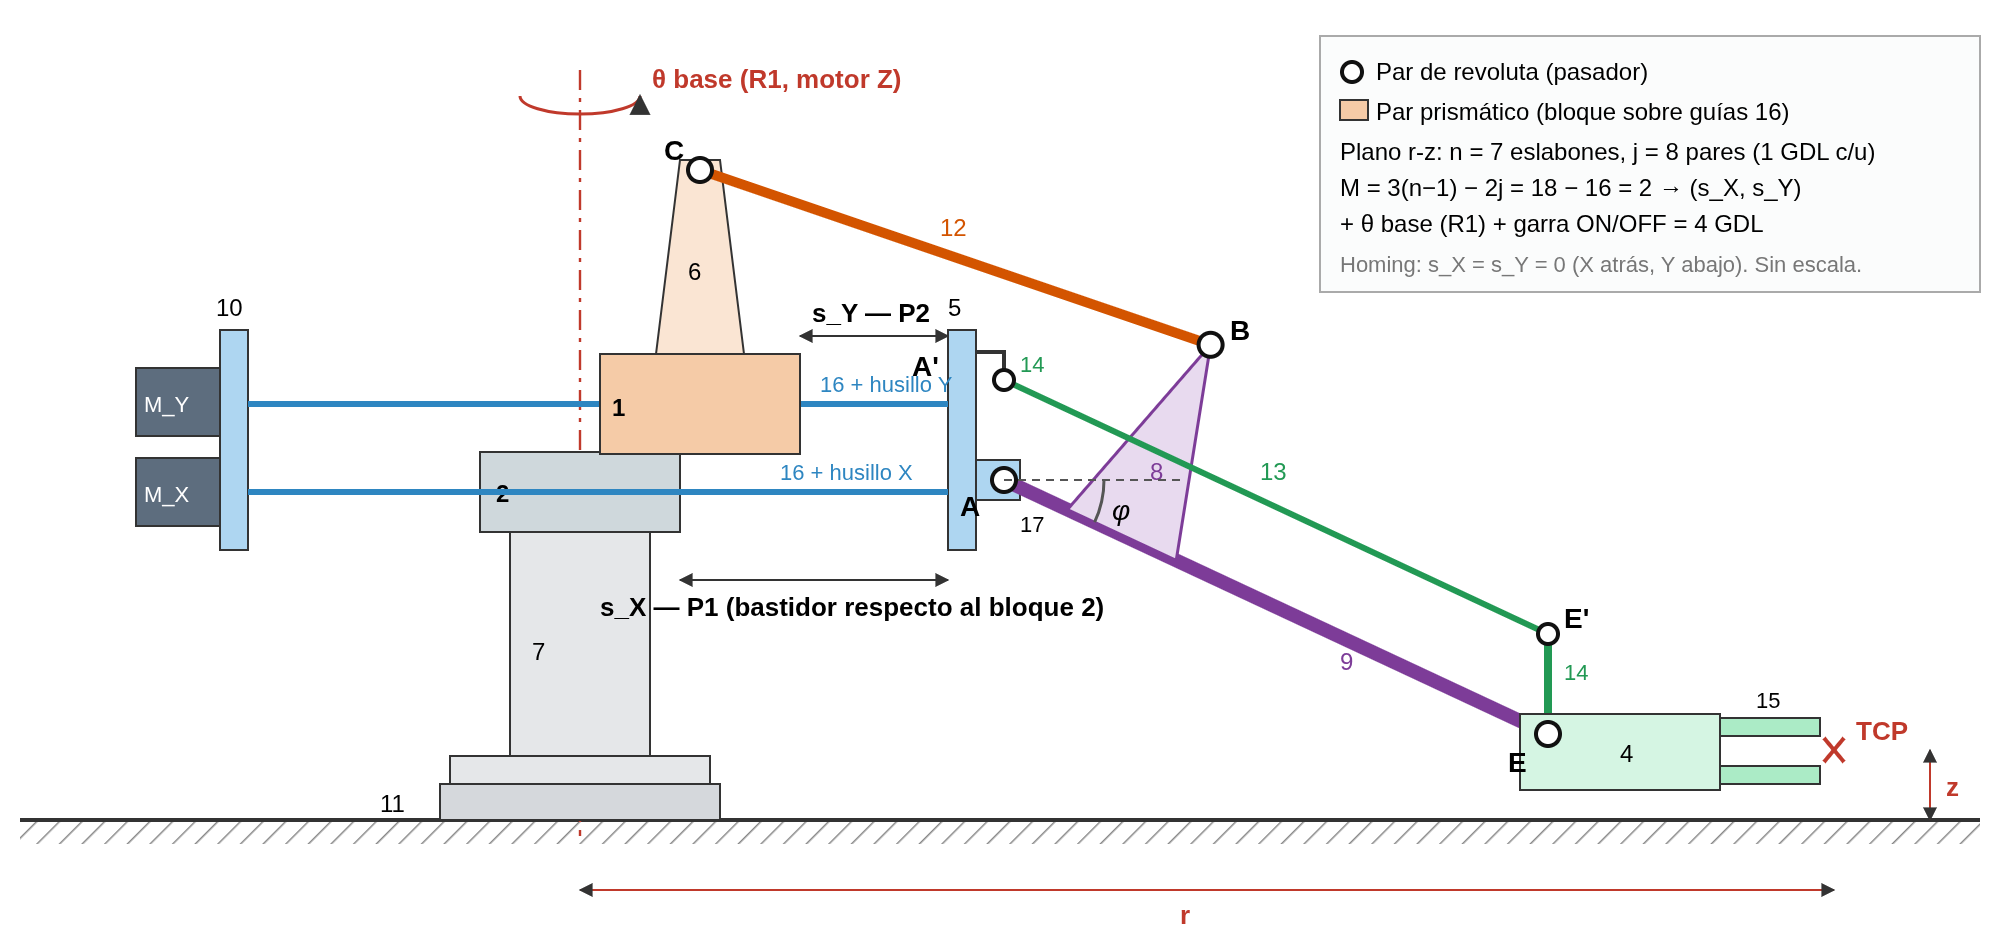
\includegraphics[width=\linewidth]{esquema_cinematico.png}
\caption{Esquema cinemático del brazo (\texttt{modelo-3d/informe/figuras/}).}
\end{figure}

El brazo trabaja en un plano vertical $(r, z)$ que gira con la base:
\begin{itemize}
\item el \textbf{carro X} desplaza todo el bastidor, y con él el pivote A del brazo: cambia el alcance;
\item el \textbf{carro Y} mueve el bloque 1 sobre el bastidor; la biela $L_{12}$ une el pivote C del bloque con el pivote B del balancín A--B, solidario al brazo: al moverse el bloque, el brazo gira un ángulo $\varphi$;
\item la varilla 13 forma un paralelogramo que mantiene la garra horizontal.
\end{itemize}

\begin{figure}[H]
\centering
\begin{tikzpicture}[x=1.05cm,y=1.05cm]
\coordinate (A) at (0,0); \coordinate (B) at (1.6,-1.0); \coordinate (C) at (4.3,-0.2);
\coordinate (E) at (6.2,2.3); \coordinate (T) at (7.6,2.0);
\draw[fill=gris] (-2.4,-2.6) rectangle (3.6,-1.9); \node[font=\scriptsize] at (0.6,-2.25) {carro X: desplaza todo el bastidor};
\draw[fill=naranja!20] (3.0,-1.0) rectangle (5.3,0.3); \node[font=\scriptsize] at (4.15,-1.4) {bloque del carro Y};
\draw[ultra thick, grisos] (A) -- (B) node[midway, left, font=\scriptsize]{$a$};
\draw[ultra thick, naranja] (B) -- (C) node[midway, below, font=\scriptsize]{$L_{12}$};
\draw[ultra thick, black] (A) -- (E) node[midway, above left, font=\scriptsize]{brazo $L_9$};
\draw[ultra thick, black] (E) -- (T);
\fill[naranja] (T) circle (0.12); \node[font=\scriptsize, right] at (T) {garra (TCP)};
\foreach \p in {A,B,C,E} {\fill[white] (\p) circle (0.11); \draw (\p) circle (0.11); \node[font=\scriptsize, above] at ($(\p)+(0,0.12)$) {\p};}
\draw[->] (A) ++(1.2,0) arc (0:35:1.2); \node[font=\scriptsize] at (1.6,0.45) {$\varphi$};
\draw[->] (A) ++(0.7,0) arc (0:-32:0.7); \node[font=\scriptsize] at (0.95,-0.25) {$\psi$};
\draw[<->] (3.0,0.7) -- (5.3,0.7) node[midway, above, font=\scriptsize]{$s_Y$};
\draw[<->] (-2.4,-2.9) -- (3.6,-2.9) node[midway, below, font=\scriptsize]{$s_X$};
\end{tikzpicture}
\caption{Esquema simplificado: lazo A--B--C y brazo A--E.}
\end{figure}

\section{Cinemática directa: de los carros a la garra}
Entrada $q = (\theta, s_X, s_Y)$; salida $(X, Y, Z)$ de la garra.

\paragraph{Paso 1: lazo de bielas.} La posición geométrica del bloque desde su tope trasero es $g = 170 - s_Y$ (el homing de Y deja el bloque adelante). El pivote C queda, respecto de A, en $C = (g + c_{u0},\, c_h) = (g - 252,\; 125)$. El pivote B está a distancia $a$ de A y a distancia $L_{12}$ de C: es la intersección de dos circunferencias. Con $d = |C|$,
\[
\psi = \operatorname{atan2}(c_h,\, g + c_{u0}) - \arccos\!\left(\frac{a^2 + d^2 - L_{12}^2}{2\,a\,d}\right),
\]
eligiendo el signo del montaje real (B por debajo de la recta A--C). El ángulo del brazo es $\varphi = \psi - \beta$.

\paragraph{Paso 2: posición de la garra en el plano.}
\[
r = u_0 + s_X + u_A + L_9\cos\varphi + d_g = 207 + s_X + 300\cos\varphi \quad [\text{mm}]
\]
\[
z = h_A + L_9\sin\varphi - h_g = 216 + 300\sin\varphi \quad [\text{mm}]
\]

\paragraph{Paso 3: giro de la base.} $X = r\cos\theta$, \ $Y = r\sin\theta$, \ $Z = z$.

\paragraph{Ejemplo resuelto: el homing $q = (0, 0, 0)$.} $g = 170$; $C = (-82, 125)$, $d = 149{,}5$~mm; $\arccos\frac{145^2 + 149{,}5^2 - 235^2}{2\cdot145\cdot149{,}5} = \arccos(-0{,}273) = 105{,}9°$; $\operatorname{atan2}(125, -82) = 123{,}3°$; $\psi = 17{,}4°$, $\varphi = -32{,}6°$. Luego $r = 207 + 0 + 300\cos(-32{,}6°) = 459{,}7$~mm y $z = 216 + 300\sin(-32{,}6°) = 54{,}4$~mm: la garra queda baja y cerca de la columna.

\begin{figure}[H]
\centering
\begin{minipage}[t]{0.49\linewidth}\centering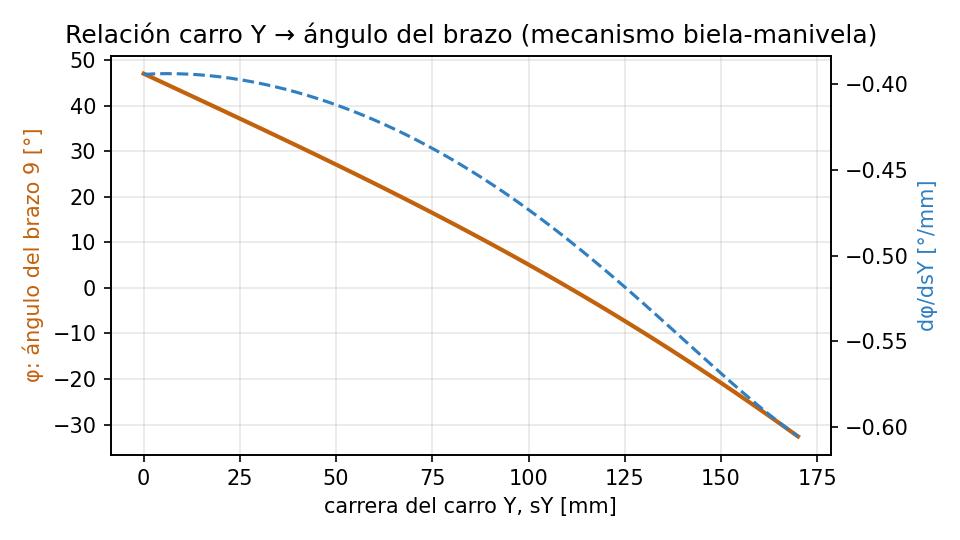
\includegraphics[width=\linewidth]{phi_vs_carro_y.png}\\{\small (a) ángulo del brazo $\varphi$ y su derivada frente a $s_Y$}\end{minipage}\hfill
\begin{minipage}[t]{0.49\linewidth}\centering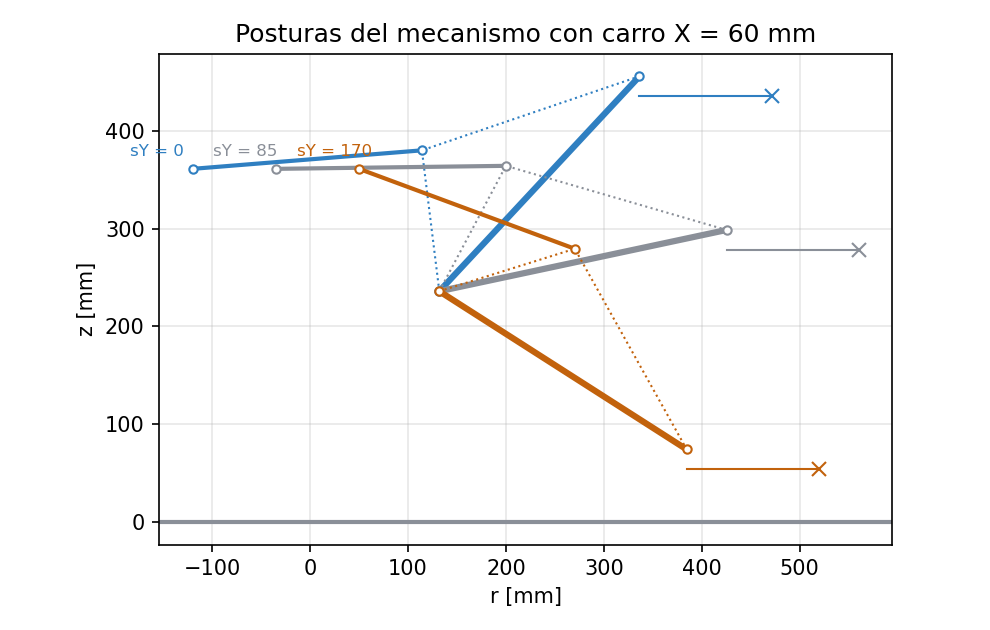
\includegraphics[width=\linewidth]{posturas_mecanismo.png}\\{\small (b) posturas del mecanismo con $s_X = 60$~mm}\end{minipage}
\caption{Relación entre el carro Y y el ángulo del brazo: de $-32{,}6°$ ($s_Y = 0$) a $+47{,}0°$ ($s_Y = 170$~mm), no lineal.}
\end{figure}

\section{Cinemática inversa: de la garra a los carros}
Entrada $(X, Y, Z)$; salida $q$.
\begin{enumerate}
\item $\theta = \operatorname{atan2}(Y, X)$, \ $r = \sqrt{X^2 + Y^2}$. Si hay varias soluciones ($\theta$ y $\theta \pm 360°$), se elige la más cercana a la actual.
\item De la altura: $\sin\varphi = \dfrac{Z + h_g - h_A}{L_9}$. Si $|\sin\varphi| > 1$, la altura es inalcanzable.
\item Del alcance: $s_X = r - d_g - L_9\cos\varphi - u_0 - u_A$.
\item Del lazo: con $\psi = \varphi + \beta$, $B = a(\cos\psi, \sin\psi)$; la biela exige $|B - C| = L_{12}$ con $C = (g - 252, 125)$:
\[
g = B_x + 252 \pm \sqrt{L_{12}^2 - (125 - B_z)^2}, \qquad s_Y = 170 - g,
\]
eligiendo la solución del montaje real.
\item Se descartan soluciones fuera de $0 \le s_X, s_Y \le 170$ o con la pinza chocando con la mesa.
\end{enumerate}

\paragraph{Ejemplo resuelto: garra en $(500, 200, 250)$~mm.} $\theta = \operatorname{atan2}(200, 500) = 21{,}80°$; $r = 538{,}52$~mm; $\sin\varphi = (250 + 20 - 236)/300 = 0{,}1133 \Rightarrow \varphi = 6{,}51°$; $s_X = 538{,}52 - 135 - 300\cos 6{,}51° - 52 - 20 = 33{,}45$~mm; $\psi = 56{,}51°$, $B = (80{,}0;\ 120{,}9)$; $g = 80{,}0 + 252 - \sqrt{235^2 - 4{,}1^2} = 97{,}05$~mm; $s_Y = 72{,}95$~mm. Comprobación con la directa: vuelve exactamente a $(500{,}000;\ 200{,}000;\ 250{,}000)$.

\section{Jacobiano y linealización}\label{sec:jacobiano}
El jacobiano relaciona pequeños movimientos de los ejes con pequeños movimientos de la garra:
\[
\Delta\mathbf{p} \approx J(q)\,\Delta q, \qquad
J = \frac{\partial(X, Y, Z)}{\partial(\theta, s_X, s_Y)} =
\begin{bmatrix}
-r\sin\theta & \cos\theta & \cos\theta\,\dfrac{\partial r}{\partial s_Y}\\[6pt]
r\cos\theta & \sin\theta & \sin\theta\,\dfrac{\partial r}{\partial s_Y}\\[6pt]
0 & 0 & \dfrac{\partial z}{\partial s_Y}
\end{bmatrix},
\]
con $\dfrac{\partial r}{\partial s_Y} = -L_9\sin\varphi\,\dfrac{d\varphi}{ds_Y}$ y $\dfrac{\partial z}{\partial s_Y} = L_9\cos\varphi\,\dfrac{d\varphi}{ds_Y}$. La derivada $d\varphi/ds_Y$ sale de derivar la ecuación del lazo $|a\,e(\psi) - C(g)|^2 = L_{12}^2$. Esta es la \textbf{linealización} del brazo alrededor de un punto de operación que pide la guía de laboratorio para la Fase 2: cerca de $q_0$, el brazo se comporta como el sistema lineal $\Delta\mathbf{p} = J(q_0)\Delta q$.

\begin{center}\small
\begin{longtable}{>{\raggedright}p{3cm} >{\centering}p{6.3cm} r r r}
\toprule
\textbf{Punto $q$} & \textbf{$J$ ($\theta$ en rad, mm/mm)} & \textbf{$\det J$} & \textbf{$d\varphi/ds_Y$} & \textbf{$\mu$}\\
\midrule
\endhead
$(0°, 0, 0)$ homing & $\begin{bmatrix}0 & 1 & 1{,}708\\ 459{,}7 & 0 & 0\\ 0 & 0 & 2{,}671\end{bmatrix}$ & 1228 & 0,606~°/mm & 37,7°\\[14pt]
$(0°, 85, 85)$ centro & $\begin{bmatrix}0 & 1 & -0{,}492\\ 585{,}4 & 0 & 0\\ 0 & 0 & 2{,}307\end{bmatrix}$ & 1350 & 0,451~°/mm & 61,3°\\[14pt]
$(30°, 120, 40)$ & $\begin{bmatrix}-311{,}3 & 0{,}866 & 0{,}411\\ 539{,}1 & 0{,}500 & 0{,}237\\ 0 & 0 & 2{,}725\end{bmatrix}$ & 1696 & 0,528~°/mm & 47,8°\\[14pt]
$(0°, 170, 170)$ esquina & $\begin{bmatrix}0 & 1 & -1{,}510\\ 581{,}5 & 0 & 0\\ 0 & 0 & 1{,}407\end{bmatrix}$ & 818 & 0,394~°/mm & 92,4°\\
\bottomrule
\end{longtable}
\end{center}

\paragraph{Cómo se lee.} En el centro $(0°, 85, 85)$: un milímetro del carro Y sube la garra 2,31~mm y la acerca 0,49~mm; un milímetro del carro X la aleja exactamente 1~mm; un grado de base la desplaza $585{,}4 \cdot \pi/180 = 10{,}2$~mm de lado. Es decir, el carro Y \emph{amplifica} su movimiento en altura por más de 2.

\paragraph{Qué tan buena es la linealización.} Comparación con la cinemática exacta desde el centro:
\begin{center}\small
\begin{tabular}{@{}lccc@{}}
\toprule
$\Delta q = (\Delta\theta, \Delta s_X, \Delta s_Y)$ & exacto $\Delta(X, Y, Z)$ [mm] & lineal $J\Delta q$ [mm] & error\\
\midrule
$(0°, 2, 2)$ & (0,98; 0; 4,59) & (1,02; 0; 4,61) & 0,04~mm\\
$(2°, 0, 0)$ & ($-0{,}36$; 20,43; 0) & (0; 20,43; 0) & 0,36~mm\\
$(0°, 10, 10)$ & (4,28; 0; 22,52) & (5,08; 0; 23,07) & 0,97~mm\\
$(5°, 0, -10)$ & (1,82; 51,38; $-23{,}61$) & (4,92; 51,09; $-23{,}07$) & 3,2~mm\\
\bottomrule
\end{tabular}
\end{center}
La aproximación es excelente para movimientos de pocos milímetros y empeora con desplazamientos grandes, sobre todo de la base (el arco no es una recta). Por eso la página recalcula la inversa en cada punto de una trayectoria en lugar de usar solo el jacobiano.

\paragraph{Singularidades y transmisión.} Como $\det J = r\,\partial z/\partial s_Y$ y en todo el recorrido $r > 400$~mm y $\partial z/\partial s_Y > 1{,}4$, el determinante nunca se anula: \textbf{no hay singularidades dentro del recorrido}. El \emph{ángulo de transmisión} $\mu$ entre la biela y el balancín (ideal 90°) mide qué tan bien la biela empuja al brazo: vale 37,7° en el homing (transmisión pobre, el carro Y necesita más fuerza) y 92,4° con el brazo arriba.

\section{Espacio de trabajo}
\begin{figure}[H]
\centering
\begin{minipage}[t]{0.56\linewidth}\centering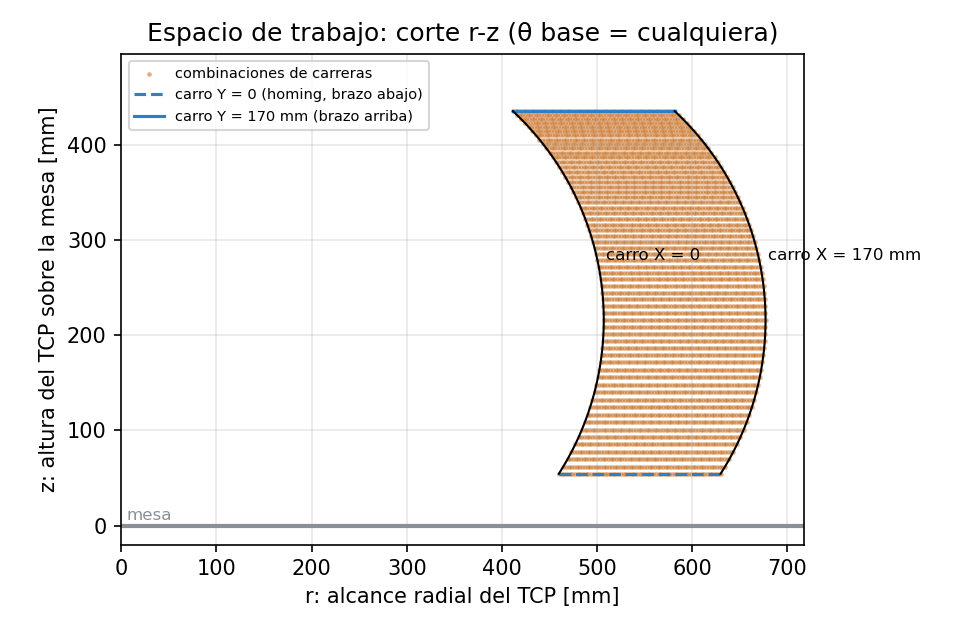
\includegraphics[width=\linewidth]{espacio_trabajo_rz.png}\\{\small (a) corte vertical $(r, z)$}\end{minipage}\hfill
\begin{minipage}[t]{0.42\linewidth}\centering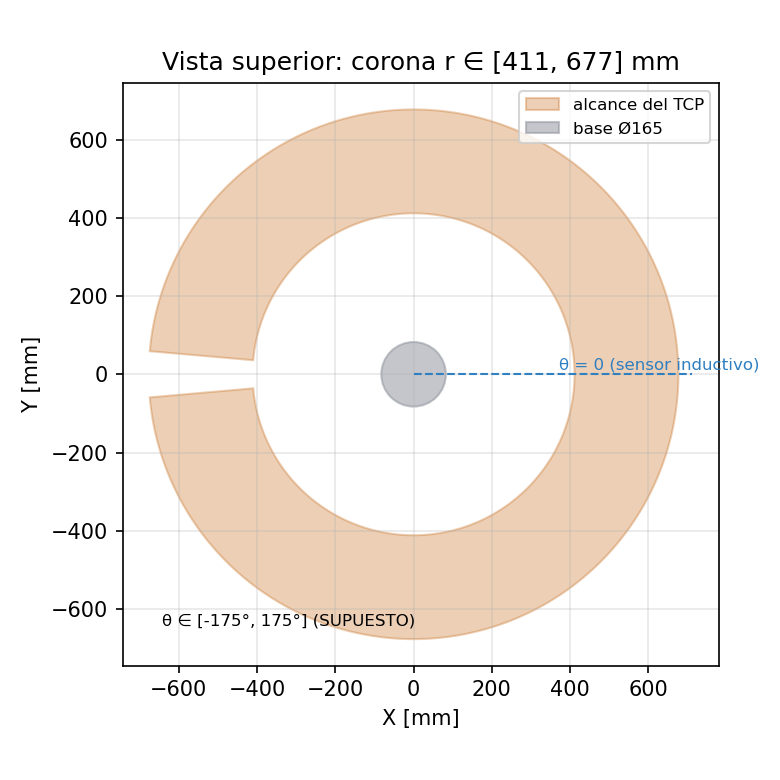
\includegraphics[width=\linewidth]{espacio_trabajo_superior.png}\\{\small (b) vista superior}\end{minipage}
\caption{Espacio de trabajo: una franja curva en el plano vertical que gira con la base; alcance radial de 411 a 677~mm.}
\end{figure}
Desde el homing (esquina inferior izquierda de la franja), un movimiento vertical de la garra sale de la zona alcanzable: por eso muchos puntos escritos a mano resultan inalcanzables, y la app propone el punto alcanzable más cercano.

\section{Modelo 3D}
Las piezas se modelaron con las mismas cotas y se ensamblaron en \codigo{global/modelo-3d/brazo\_xk-js1-1.glb}, generado por el script \codigo{generar\_modelo.js} (sin programas de diseño). El visor (three.js) coloca cada pieza según la cinemática directa en cada cuadro.

\begin{figure}[H]
\centering
\begin{minipage}[t]{0.49\linewidth}\centering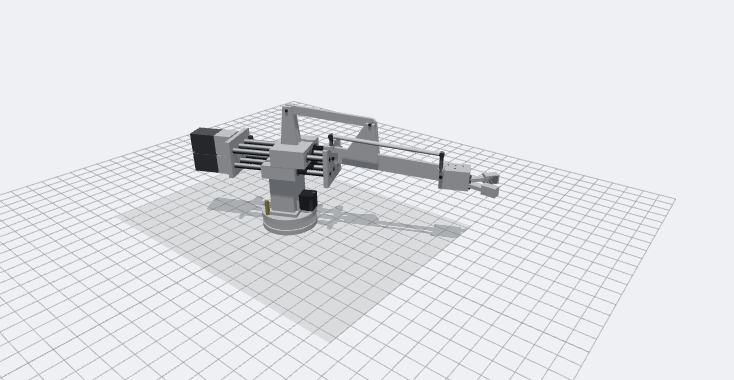
\includegraphics[width=\linewidth]{modelo_3d_isometrica.png}\\{\small (a) isométrica}\end{minipage}\hfill
\begin{minipage}[t]{0.49\linewidth}\centering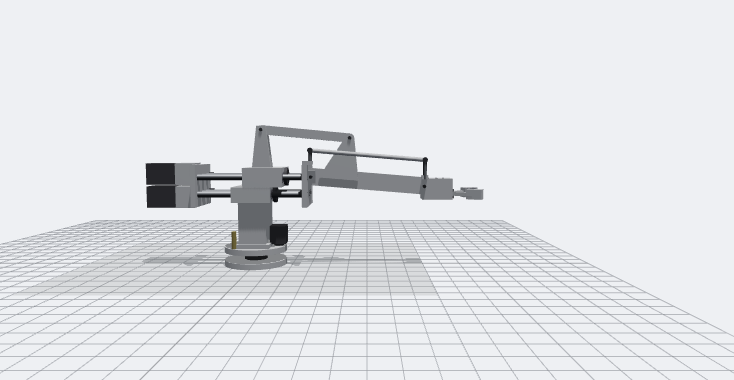
\includegraphics[width=\linewidth]{modelo_3d_lateral.png}\\{\small (b) lateral}\end{minipage}
\caption{Modelo 3D del brazo.}
\end{figure}

\section{Scripts del modelado}
\begin{center}\small
\begin{tabularx}{\linewidth}{>{\raggedright}p{6.2cm} >{\raggedright\arraybackslash}X}
\toprule
\textbf{Archivo} & \textbf{Qué hace}\\
\midrule
\codigo{web/js/cinematica.js} & modelo: parámetros, directa, inversa, jacobiano, espacio de trabajo, pulsos, trayectorias\\
\codigo{modelo-3d/cinematica/pruebas\_cinematica.js} & pruebas: la inversa de la directa devuelve el mismo $q$; exporta \codigo{parametros.json} y \codigo{tabla\_cinematica.csv}\\
\codigo{modelo-3d/cinematica/cinematica\_brazo.m} & la misma cinemática en MATLAB\\
\codigo{modelo-3d/cinematica/graficas\_cinematica.py} & gráficas del informe (espacio de trabajo, $\varphi(s_Y)$, posturas)\\
\codigo{modelo-3d/levantamiento/generar\_esquema\_medidas.py} & esquemas acotados del levantamiento\\
\codigo{global/modelo-3d/generar\_modelo.js} & genera el modelo 3D \codigo{.glb}\\
\bottomrule
\end{tabularx}
\end{center}

\begin{lstlisting}[style=js, caption={Cinemática inversa (fragmento de \texttt{web/js/cinematica.js}).}]
const s = (obj.Z + p.hg - d.hA) / p.L9;           // seno del ángulo del brazo
if (Math.abs(s) > 1) return { valida: false, motivo: 'Altura inalcanzable' };
for (const [rama, phi] of [['adelante', Math.asin(s)], ['atrás', Math.PI - Math.asin(s)]]) {
  const sX = r - p.dg - p.L9 * Math.cos(phi) - d.u5_0 - p.uA;   // alcance -> carro X
  const psi = phi + beta;                                         // balancín A-B
  const bx = p.a * Math.cos(psi), bz = p.a * Math.sin(psi);
  const disc = p.L12 * p.L12 - (d.ch - bz) * (d.ch - bz);         // biela L12 hasta C
  if (disc < 0) continue;
  // dos posiciones posibles del bloque; se queda la del montaje real
}
\end{lstlisting}
